\chapter{Proposta per un iter autorizzativo} %\label{1cap:spinta_laterale}

\begin{preamble}
In questo capitolo conclusivo si cercherà di proporre una procedura di autorizzazione armonica e collegata a quanto emerso nello studio della geotermia a bassa entalpia. Non saranno quindi presi in considerazione le perforazioni geotermiche di profondità, perché esulano dallo scopo del testo e la loro autorizzazione deve essere esaminata caso per caso, mentre le sonde orizzontali e le fondazioni energetiche, pur rientrando nella categoria saranno tralasciate, perché le prime hanno un impatto ambientale trascurabile e sono già regolamentate negli scavi e ripristini per la posa di reti ed impianti e le seconde invece richiedono una progettazione termica/strutturale specialistica.

Per i sistemi a circuito aperto e chiuso si consiglieranno allora i compiti e le procedure che l'ente di controllo dovrebbe svolgere per concedere l'autorizzazione e la vigilanza degli impianti geotermici e la documentazione che la potenziale committenza dovrebbe fornire per descrivere l'impianto e per mitigare l'impatto ambientale.

Infine si riporteranno alcuni utili consigli che possono essere prescritti dall'ente di controllo e seguiti dal committente in fase di progettazione, per ridurre l'impatto ambientale da un lato e risparmiare sui costi di perforazione e gestione dall'altro.
\end{preamble}

\section{Competenze dell'ente di controllo}
Ferme restando norme e misure evidenziate nel capitolo ref{6cap:regolamenti} che fissano e definiscono gli enti preposti per rilasciare l'autorizzazione e tutelare le acque sotterranee, si tratta ora di prendere in considerazione i principi e le misure di vigilanza da intraprendere per la sostenibilità ambientale degli impianti geotermici. Gli enti di controllo (Regione e Provincia), dovrebbero seguire due orientamenti strettamente collegati tra loro e così riassumibili:
\begin{itemize}
\item pianificazione territoriale geotermica;
\item disciplinare per un utilizzo congruo della risorsa.
\end{itemize}

Un sistema realizzato a regola d'arte non costituisce un pericolo ambientale, in quanto la terebrazione di pozzi e la trivellazione sono opere ampiamente definite e normate. Si è visto però che il calore trasferito ed il fattore tempo giocano un ruolo fondamentale, sia nella definizione del bacino termico del terreno, sia nel dimensionamento dell'impianto. La perturbazione termica causata a breve e/o a lungo termine infatti potrebbe arrecare danno all'ambiente e alle utilizzazioni circostanti e ridurre le prestazioni della pompa di calore per l'utenza.

Alla definizione della perturbazione termica concorrono molti fattori, tra i quali: i carichi termici annuali dell'edificio, le proprietà termiche del terreno, la velocità e la direzione della falda sotterranea e la sovrapposizione di altri sistemi geotermici operanti nella zona. Fattori che non possono essere tralasciati in fase di concessione dell'autorizzazione e che dovrebbero poi andare a costituire un database cartografico di facile consultazione.

Inoltre un uso improprio della risorsa, per la variazione dei carichi di riscaldamento o raffrescamento annuali ipotizzati in fase di progetto, può allo stesso modo causare gravi deficit all'impianto e al territorio circostante. Per questo motivo, come già viene fatto per le consuete licenze, è consigliabile rilasciare un disciplinare con clausole e condizioni d'uso della geotermia.

Nel rilascio delle concessioni\index{concessioni} infine è preferibile privilegiare sistemi geotermici che sono progettati per la climatizzazione annuale degli edifici (cioè con carichi grossomodo bilanciati tra la stagione invernale ed estiva) ed eventuali sistemi ibridi (cioè integrati con sistemi di climatizzazione tradizionali per coprire i carichi di picco). In questo modo il sottosuolo mantiene una temperatura costante nella vita utile dell'impianto e quindi l'impatto ambientale si minimizza.

\begin{figure}[h]
	\centering
	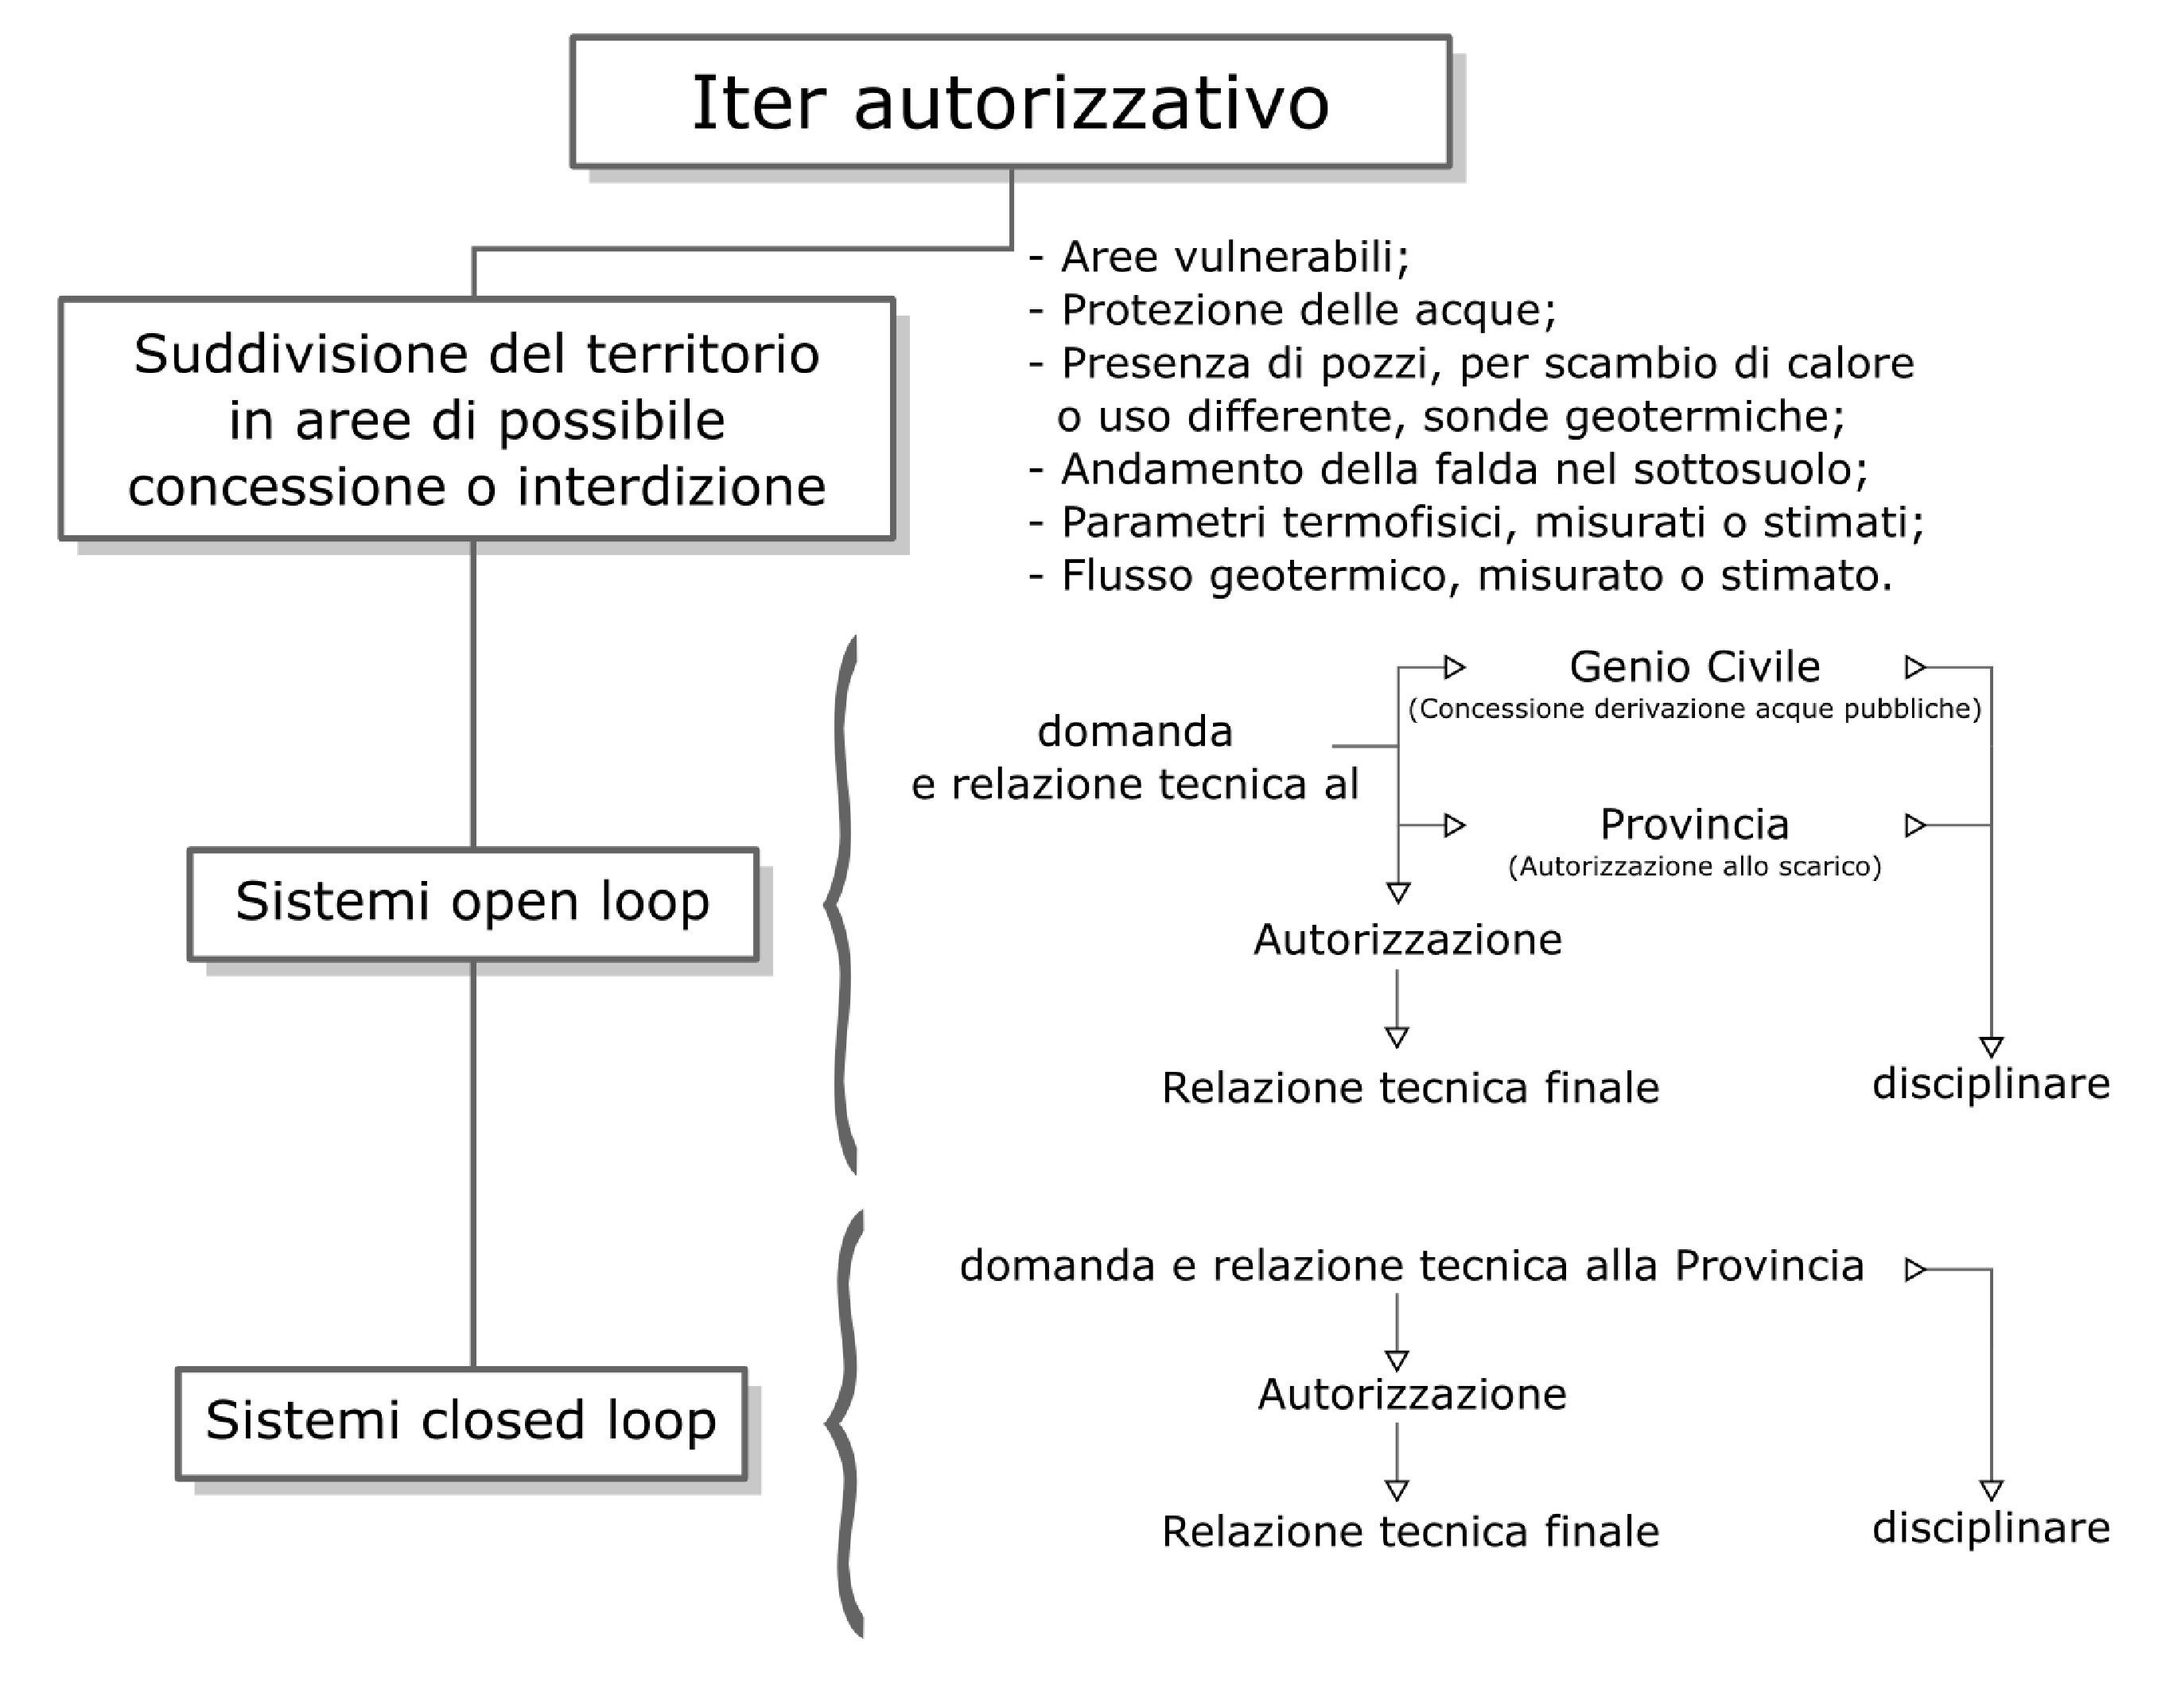
\includegraphics [width=.95\columnwidth, angle=0]{iter_autorizzativo} % height
	\caption{Possibile schema di un iter autorizzativo per i sistemi a circuito aperto e chiuso}
	\label{8fig:iter_autorizzativo}
\end{figure}

\subsection{Pianificazione territoriale}
L'ente di controllo, avvalendosi di una pianificazione del territorio che tenga in considerazione non solo le aree sensibili e di ricarica delle falde, ma anche la presenza di impianti di captazione e geotermici (con la loro impronta idraulica e termica), può autorizzare e inibire l'installazione di nuovi impianti o il loro eventuale ampliamento. Allo scopo sono stati riportati ed elencati software di modellazione numerica delle falde (sottoparagrafo vref{3subsec:modellazionefalde}) e dei campi sonde (paragrafo vref{4sec:grandiimpianti}), che possono essere di aiuto non solo nella progettazione ma anche nelle gestione dinamica e del sottosuolo su piccola e media scala.

Tutto questo lavoro di programmazione e progettazione territoriale può sembrare oneroso e superfluo, per una tecnologia che allo stato attuale è ancora sconosciuta in Italia, ma può rappresentare una soluzione obbligata per l'abbattimento dei costi per la climatizzazione degli edifici e delle emissioni di CO\ped{2} nei prossimi anni. Una autorizzazione limitata alla sola protezione della risorsa idrica nel sottosuolo, può portare alla saturazione e alla sovrapposizione di serbatoi geotermici, se la tecnologia dovesse diventare popolare in tempi brevi e sostituire l'impiantistica tradizionale.

\subsection{Disciplinare}
Una volta concessa l'autorizzazione per l'installazione dell'impianto, l'ente di controllo, nell'usuale disciplinare che regola le clausole e le condizioni d'uso della risorsa, dovrebbe stabilire inoltre la quantità di calore da derivare (media e di picco) e la durata della concessione con modalità e termini per il rinnovo.

\section{Competenze del committente}
Realizzare un sistema geotermico è attualmente oneroso e richiede una progettazione specialistica che pochi installatori possono assicurare o certificare. Il costo iniziale poi è più elevato degli impianti tradizionali e richiede la redazione di relazioni tecniche e idrogeologiche che interessano molteplici figure professionali, sia per il dimensionamento dell'impianto, sia per ottenere la concessione.

\'E bene esserne consapevoli e ricorrere a questo tipo di soluzione per impianti di una certa importanza e che possano servire più utenze. In questo modo si possono ridurre i costi ottimizzando le perforazioni e la gestione del sottosuolo e si possono prevedere analisi e progettazioni più dettagliate.

Inoltre un dimensionamento ottimale dei fabbisogni termici può contribuire a ridurre gli interventi sul terreno che rappresentano la parte più significativa del costo dell'impianto. Vale la pena poi considerare nell'analisi costi/benefici, l'installazione di un sistema ibrido per coprire il carico di picco, se quest'ultimo si raggiunge per poche ore all'anno e far coprire al sistema geotermico il restante \numprint[\%]{90} dell'energia termica richiesta.

Seguendo ed integrando quanto proposto da \cite{anipa}, la committenza per ottenere l'autorizzazione alla realizzazione degli impianti geotermici, dovrà produrre una:
\begin{itemize}
\item domanda da presentare agli organi competenti;
\item relazione idrogeologica preliminare;
%\item competenza della direzione lavori;
\item relazione idrogeologica finale.
\end{itemize}

Di seguito verranno schematizzati i contenuti base di queste domande e relazioni, suddividendole per tipo di impianto ed elencando le competenze della direzione lavori. Ovviamente gli enti di controllo richiederanno maggiori richieste, prescrizioni ed integrazioni a quanto sommariamente elencato. Qui si vuole solo fornire un quadro sintetico e generale, con evidenziate le richieste utili per richiedere ed agevolare l'autorizzazione.

\newpage
\section{Domanda e relazione tecnica preliminare}
La domanda per i due sistemi comprenderà:
\begin{itemize}
\item dati anagrafici del richiedente;
\item dati del progettista e della Direzione Lavori (se differente);
\item dati indicativi della ditta e/o ditte (con eventuali certificazioni);
\item dati significativi dell'impianto (perforazione e installazione);
\item dati indicativi sull'ubicazione dell'impianto.
\end{itemize}

Dovranno poi essere allegati:
\begin{itemize}
\item relazione tecnica di progetto;
\item corografia ubicativa 1:\numprint[]{25000} e planimetria catastale 1:\numprint[]{2000}; 
\end{itemize}

\begin{table}[h]%\footnotesize
	\caption{Requisiti dell'acqua estratta per gli impianti open loop \citep{uni_15450}}
	\label{2tab:valori_richiesti_pdc}
	\centering
	\rowcolors{2}{gray!25}{}
%	\resizebox{0.95\columnwidth}{!}{%
	\begin{tabular}{>{\bfseries}lcc}
	\toprule
componenti		&	valore 		&	unità di misura 	\\
	\midrule
materiale organico	(possibilità di sedimentazione)	&	nessuna		&	-	\\
valore di pH		&	$6,5 \div 9$		&	-	\\
conduttività elettrica		&	$50 \div \numprint[]{1000}$		&	$ \mu \: \mathrm{S} \: \mathrm{cm^{-1}}$	\\
cloruro		&	$< 300$		&	$\mathrm{mg} \: \mathrm{\ell^{-1}}$	\\
ferro e manganese		&	$<1$		&	$\mathrm{mg} \: \mathrm{\ell^{-1}}$	\\
solfato		&	$<2$		&	$\mathrm{mg} \: \mathrm{\ell^{-1}}$ \\
contenuto di O\ped{2}		&	$<2$		&	$\mathrm{mg} \: \mathrm{\ell^{-1}}$	\\
cloro		&	$0\div5$		&	$\mathrm{mg} \: \mathrm{\ell^{-1}}$	\\
nitrato		&	$0\div100$	&	$\mathrm{mg} \: \mathrm{\ell^{-1}}$	\\
	\bottomrule
	\end{tabular}%}
\end{table}

\subsection{Per sistemi open loop}
La relazione tecnica comprenderà:
\begin{description}
\item[$\blacktriangleright$] Dati tecnici
\begin{itemize}
\item potenza dell'impianto ($\mathrm{kW\ped{t}}$);
\item fabbisogno termico mensile, con carico medio e di picco;
\item portata necessaria ($\mathrm{m\ap{3}s\ap{-1}}$);
\item $\Delta \mathrm{T}$ (K o $\celsius$);
\item dotazioni di sicurezza e controllo.
\end{itemize}
\item[$\blacktriangleright$] Dati idrogeologici
\begin{itemize}
\item controllo dei vincoli esistenti nell'area di indagine;
\item inquadramento geologico;
\item idrogeologia del sottosuolo (caratteristiche dell'acquifero, permeabilità e direzione di flusso);
\item censimento dei pozzi esistenti nell'area e di altre perforazioni:
\item analisi qualitativa dell'acqua prelevata e restituita alla falda.
\end{itemize}
\item[$\blacktriangleright$] Progetto
\begin{itemize}
\item schema di progetto per la costruzione dei pozzi, con particolare riferimento a diametri e materiali di filtri e rivestimento;
\item descrizione sulle metodologie previste per eseguire a regola d'arte la cementazione del foro;
\item valutazioni sulle possibili conseguenze relative al prelievo dell'acqua e sulla reimmissione, indicando il $\Delta T$ previsto a breve e a lungo termine (il massimo ammesso è di \numprint[\tccelsius]{5}) e la compatibilità ambientale dello scarico nel corpo recipiente.
\end{itemize}
\end{description}

\newpage
\subsection{Per sistemi closed loop}
La relazione tecnica comprenderà:
\begin{description}
\item[$\blacktriangleright$] Dati tecnici
\begin{itemize}
\item potenza dell'impianto (kW\ped{t});
\item fabbisogno termico mensile, con carico medio e di picco;
\item fluidi, additivi e anticongelanti che verranno utilizzati;
\item $\Delta \mathrm{T}$ (K o $\celsius$);
\item dotazioni di sicurezza e controllo.
\end{itemize}
\item[$\blacktriangleright$] Dati idrogeologici
\begin{itemize}
\item controllo dei vincoli esistenti nell'area di indagine;
\item inquadramento geologico;
\item idrogeologia del sottosuolo (caratteristiche dell'acquifero o degli acquiferi attraversati, permeabilità e direzione di flusso);
\item censimento dei pozzi esistenti nell'area e di altre perforazioni.
\end{itemize}
\item[$\blacktriangleright$] Progetto
\begin{itemize}
\item schema di progetto per la costruzione della sonda o del campo sonde;
\item indicazioni specifiche sulla metodologia di perforazione e sui relativi diametri;
\item descrizione sulle metodologie previste per eseguire a regola d'arte la cementazione del foro.
\item simulazione degli effetti con definizione del tipo, della localizzazione e della quantità della perturbazione termica, a breve e a lungo termine. 
\end{itemize}
\end{description}

\subsection{Compiti della direzione lavori}
Dovrà verificare la corretta esecuzione della posa in opera e controllare che in fase di perforazione la stratigrafia (i cui campioni dovranno essere lasciati a disposizione delle autorità competenti), sia corrispondente a quella prevista in fase di progetto ed in caso contrario predisporre delle adeguate soluzioni tecniche per mitigare le novità emerse.

Dovrà verificare con particolare attenzione gli aspetti relativi alla cementazione, dovendone certificare poi la tenuta. Inoltre eseguirà a seconda dell'impianto realizzato:
\begin{itemize}
\item prova di verifica a pressione della tenuta;
\item prova di portata nel pozzo di presa e di immissione in quello di scarico.
\end{itemize}

\newpage
\section{Relazione tecnica finale}
\subsection{Per sistemi open loop}
Comprenderà:
\begin{itemize}
\item dati stratigrafici effettivi;
\item schema effettivo dei pozzi realizzati;
\item dati idrogeologici derivanti anche dai risultati delle prove di pompaggio eseguite;
\item valutazioni sulle possibili conseguenze del prelievo e della restituzione;
\item calcolo dell'area influenzata dal $\Delta T$ nel breve e lungo termine (bulbo termico).
\end{itemize}

Verrà allegata:
\begin{itemize}
\item la planimetria con le effettive ubicazioni dei pozzi eseguiti con evidenziato il raggio di influenza del $\Delta T$ a breve e lungo termine.
\end{itemize}

La D.L. attesterà mediante dichiarazione sottoscritta la tenuta della cementazione, dell'impianto, la non interferenza tra le falde eventualmente presenti sia tra loro che con la superficie e la compatibilità ambientale dello scarico nel corpo recipiente.

\subsection{Per sistemi closed loop}
Comprenderà:
\begin{itemize}
\item dati stratigrafici effettivi;
\item schema effettivo dei pozzi realizzati;
\item variazioni rispetto al progetto preliminare;
\item dati relativi alla cementazione eseguita;
\item simulazione effettiva degli effetti con definizione del tipo, della localizzazione e della quantità della perturbazione termica, a breve e a lungo termine.
\end{itemize}

Verrà allegata:
\begin{itemize}
\item la planimetria con le effettive ubicazioni delle sonde eseguite e la perturbazione termica, a breve e a lungo termine.
\end{itemize}

La D.L. attesterà mediante dichiarazione sottoscritta la tenuta della cementazione e dell'impianto e la non interferenza tra le falde eventualmente presenti, sia tra loro che con la superficie.